% DespachoX · manuscript draft v0.1 (English)
% Branch: manuscrito · Folder: docs/manuscrito/
% Compile: nice -n 19 latexmk -lualatex main.tex
%
% Conventions used in this draft
%   [SIM]              number pending from the simulation run of 21 November 2026 (results expected ~6 a.m.)
%   [SIM-CONFIG]       design detail of that run that must be checked against its configuration
%   [MISSING SOURCE]   claim kept in the text whose source we could not find
%   \cite{PORVERIFICAR_<key>}  reference that could not be verified; listed in CITAS_POR_VERIFICAR.md.
%                      It prints as "(?)" on purpose.
%   % CODE-vs-DOC      comment that records a disagreement between the code and the team's documentation;
%                      the text follows the code.
% Style: Carlos's rules for academic texts (one idea per sentence, no em dashes for asides, no
% "not X but Y", no aphorisms at the end of paragraphs, no crutch words). Keep them when editing.

\documentclass[11pt]{article}

\usepackage[a4paper,margin=2.5cm]{geometry}
\usepackage{fontspec}
\usepackage[english]{babel}
\usepackage{microtype}
\usepackage{amsmath,amssymb,mathtools}
\usepackage{booktabs,tabularx,array,longtable}
\usepackage[flushleft]{threeparttable}
\usepackage{enumitem}
\usepackage{xcolor}
\usepackage{graphicx}
\usepackage{tikz}
\usetikzlibrary{arrows.meta,positioning,fit,calc,backgrounds}
\usepackage[round,authoryear]{natbib}
\usepackage[font=small,labelfont=bf]{caption}
\usepackage{xurl}
\usepackage[hidelinks]{hyperref}

\linespread{1.12}
\setlist{itemsep=2pt,topsep=4pt}
\newcolumntype{L}[1]{>{\raggedright\arraybackslash}p{#1}}
\newcolumntype{Y}{>{\raggedright\arraybackslash}X}

% Pending material is printed in dark red so that it cannot be mistaken for a result.
\newcommand{\pend}[1]{\textcolor{red!60!black}{#1}}
\newcommand{\code}[1]{\texttt{\small #1}}
\newcommand{\cS}{\mathcal{S}}

\title{DespachoX: a human-approved dispatch desk for food aid under road closures in Manizales, Colombia}
\author{Authors to be determined}
\date{Draft v0.1, 21 November 2026}

\begin{document}
\maketitle

\begin{center}
\fbox{\parbox{0.92\linewidth}{\small
\textbf{Draft notice.} Numbers marked \pend{[SIM]} will come from the simulation run of 21 November 2026; no earlier simulation result is used in this draft. Citations printed as ``(?)'' are pending verification and are listed in \code{CITAS\_POR\_VERIFICAR.md}. Press and government figures were retrieved on 20 and 21 November 2026 and still need to be opened by a member of the team, as the team's own rule requires. Not for circulation.}}
\end{center}

\begin{abstract}
\noindent
Food aid converged on Manizales, Colombia, after the earthquake of 10 August 2026. On the sixth day, the national network of food banks reported 404,587\,kg held in its collection centres and 41,163\,kg delivered. Dispatching in this hillside city has to reconcile requests that arrive as free text, roads that landslides close during the day, and perishable stock with uneven expiry dates. DespachoX is a dispatch desk built on one rule. A language model reads and structures messages. An optimizer and explicit rules compute plans. A named dispatcher approves every plan before anything moves. Requests and road reports arrive by chat or, when mobile data fail, by text messages parsed by rules. A routing model assigns orders to a mixed fleet, with one road network per vehicle type, expiry as a hard deadline and lateness weighted by urgency, and is solved again after each confirmed closure. Each package carries a code until someone confirms its delivery. We state the model as implemented and compare it, in a discrete-event simulation on the road network of Manizales, with first-come-first-served dispatch and with an expert rule that serves urgent orders and earliest-expiring stock first. \pend{[SIM]: main finding in one sentence, with at most two figures.} Demand, inventory, fleet and closures in the simulation are synthetic, and most operating parameters are assumptions. A pilot with the city's food bank is designed to measure the effect on real operations.
\end{abstract}

\noindent\textbf{Keywords:} humanitarian logistics; last-mile distribution; vehicle routing; road closures; perishable food; human-in-the-loop decision support; large language models; Colombia.

% ======================================================================================
\section{Introduction}\label{sec:intro}

The earthquake of 10 August 2026 had magnitude 7.4 and its epicentre in San José del Palmar, Chocó. The national government declared a state of emergency in fifteen departments, Caldas among them \citep{decreto2026emergencia}. In Manizales, the capital of Caldas, the census that closed on 24 August registered 8,240 affected people and 3,080 evacuated properties \citep{rcn2026demolicion}. Food aid arrived quickly. The national network of food banks, ABACO, opened a humanitarian corridor on the day of the earthquake, and Manizales became one of its main collection points \citep{rcn2026corredor}. Six days later the food banks reported 41,163\,kg of aid delivered, 157,164\,kg in transit and 404,587\,kg still held in collection centres \citep{portafolio2026flypass}.

Supplies that accumulate faster than they can be distributed are a recurrent feature of disasters. \citet{holguinveras2014material} call the spontaneous inflow of goods into an affected area material convergence, and they document how its non-priority part complicates relief operations. Post-disaster logistics also differs from commercial logistics in its objectives, its information and the people who run it \citep{holguinveras2012unique}. The figures above suggest that in August 2026 the binding constraint lay downstream of the donation, in the step that turns stock into deliveries. This is our reading of press figures, and the pilot in Section~\ref{sec:pilot} is designed to test it.

Dispatching food in Manizales is hard for reasons that predate the earthquake. The city lies on a mountain ridge, and most of its access roads run along slopes. Landslides close them in ordinary rainy seasons \citep{ani2021cierre,invias767}. Whoever decides each morning what leaves a warehouse, for whom, in which vehicle and by which road works with inputs that change during the day. Requests arrive as free text by telephone and chat, often duplicated, with places named the way residents name them. Drivers learn of a closure before any registry does. Part of the stock is perishable, so the order in which lots leave the warehouse decides how much of it is lost. Each of these difficulties has known partial remedies. We hypothesize that their combination, under time pressure and with volunteers who may have arrived the day before, is where manual dispatch fails.

DespachoX is a dispatch desk built for that combination. Its design follows one rule that the team treats as non-negotiable. A language model reads and structures messages. An optimizer and explicit rules compute. A human dispatcher decides. Neighbourhood committees request food by chat or text message, and drivers report blocked roads through the same channels. Rules allocate the stock that expires first, and an optimizer assigns the orders to a mixed fleet of trucks, four-wheel-drive vehicles and motorcycles. The plan is recomputed whenever a closure is confirmed. Each package carries a code from the warehouse to the confirmation of delivery. The dispatcher approves every plan under their own name, and the system records each decision.

The project began at the hackathon of Universidad Nacional de Colombia in Manizales, on 20 and 21 November 2026, in a challenge on logistics and supply. The challenge asked for a real-time dispatch platform or protocol with route optimization and traceability of aid packages, for a mixed fleet. It fixed two indicators, which this paper adopts as its primary outcomes: the share of deliveries at critical points made on time, and the waste of perishable food, to be kept below 5\%. % Source: challenge card of vertical 04 on the hackathon website (summarized in docs/ESTRATEGIA.md, section 2). Cite the website if the venue allows it.

The routing algorithm in DespachoX is standard. The contribution lies in joining intake, dispatch, re-planning and traceability in one flow under explicit human control, and in measuring that flow with declared assumptions. In our review of tools and of the 2026 press coverage, we found no open tool that joins a chat request, a mixed-fleet dispatch aware of expiry and closures, and a confirmed delivery (Section~\ref{sec:related}). That review was not systematic, so the finding holds only for what we searched.

Four parts of the work can be checked independently. The architecture rule is stated as a design principle, with each human gate placed in the data flow (Section~\ref{sec:system}). The optimization model is written down as the code implements it, including the points where code and documentation disagree (Section~\ref{sec:model}). The simulation protocol uses common random numbers and two baselines, one of which imitates an experienced dispatcher, because simple practice-based rules can perform close to optimized plans \citep{cook2017dispatching,gralla2018humanitarian} (Section~\ref{sec:simdesign}). The pilot measures the system against the food bank's own operation for up to 90 days, in a named territory, during the recovery phase (Section~\ref{sec:pilot}).

% ======================================================================================
\section{Related work}\label{sec:related}

\subsection{Objectives for last-mile relief distribution}

Research on last-mile relief distribution has moved away from cost as the main objective. \citet{campbell2008routing} compared relief routing with minimum-cost routing and proposed minimizing the maximum or the average arrival time. \citet{huang2012relief} separated efficiency, efficacy and equity as objectives and examined how each of them shapes the structure of the routes. \citet{balcik2008lastmile} decided the allocation of supplies and the vehicle routes jointly, with equity among recipients in the objective. \citet{holguinveras2013objective} argued that the appropriate objective is social cost, the sum of logistic costs and deprivation costs. \citet{holguinveras2016deprivation} later estimated deprivation cost functions for drinking water through a contingent valuation experiment. Reviews by \citet{anayaarenas2014relief} and \citet{delatorre2012disaster} cover relief distribution networks and the distance between routing research and field practice, and \citet{beamon2008performance} discuss how performance should be measured in relief chains.

DespachoX does not estimate deprivation costs. Its objective is a declared surrogate: travel time, plus lateness weighted by urgency, plus a large penalty for each order left unserved (Section~\ref{sec:model}). Equity is reported as an outcome, the waiting time of the worst-served point, and has no term in the objective.

\subsection{Dynamic routing on damaged networks}

Relief routing is dynamic because requests, supplies and road conditions change while vehicles are on the road. \citet{ozdamar2004emergency} re-solved a multi-period transportation model at regular intervals as new requests, supplies and vehicles became known. \citet{pillac2013review} review dynamic vehicle routing more broadly. When the network itself is uncertain, information about damage has value of its own. \citet{escribanomacias2020endogenous} use unmanned aerial vehicles to reveal the state of the network before ground vehicles distribute relief. DespachoX relies on cheaper sensors. Drivers report the closures they find, a dispatcher confirms them, and the routing problem is solved again from the vehicles' current positions.

\subsection{Practice-based rules as baselines}

Intuitive dispatch rules are serious competitors for any optimizer. \citet{cook2017dispatching} compared heuristic dispatching policies with an optimal policy obtained by stochastic dynamic programming, for a relief chain with uncertain supply and demand, and found the simple policy optimal or close to optimal in most situations. \citet{gralla2018humanitarian} built heuristics that mirror how humanitarian organizations plan transportation, compared them with a mixed-integer program, and found that a simple practice-driven heuristic performs well when deliveries are prioritized by destination priority or by distance. They suggest that automating such a heuristic in a decision support tool can keep its simplicity and transparency. In Colombia, \citet{rueda2021coordinacion} identified sixteen priority rules that field actors use to distribute aid in the last mile, five of which account for 78\% of their decisions. These findings shape our evaluation. Its demanding baseline imitates an experienced dispatcher who serves urgent orders first and releases the earliest-expiring stock first (Section~\ref{sec:simdesign}).

\subsection{Perishable food}

One line of work models perishability in routing as a cost incurred during delivery. \citet{hsu2007vehicle} extended the vehicle routing problem with soft time windows to perishable food, with inventory and energy costs and with temperatures that vary during the day. DespachoX uses a simpler representation. The expiry of each lot is a hard deadline on arrival, and stock rotation is a rule applied before routing (Section~\ref{sec:model}). Rotation matters in this setting. In August 2026 the executive director of ABACO pointed to power cuts that prevented a cold chain for some foods, and to canned food that can be opened and eaten immediately \citep{larepublica2026abaco}.

\subsection{Crisis messages, crowdsourcing and language models}

Turning crisis messages into structured requests predates large language models. After the 2010 earthquake in Haiti, Mission 4636 relied on volunteers to translate, categorize and geolocate text messages sent by the affected population \citep{munro2013crowdsourcing}. AIDR classified crisis messages in real time with machine learning trained on labels provided by people \citep{imran2014aidr}, and \citet{imran2016twitter} released human-annotated tweets from crises of 2013 to 2015 in English, Spanish and French. Current models still behave unevenly. Zero-shot classification of crisis tweets by three commercial models varied considerably across datasets \citep{mcdaniel2024zeroshot}. A robustness study of six models found that they struggle most with urgent requests and needs, that typing errors degrade them, and that adding examples to the prompt helps little \citep{imran2025robustness}. A study by The Engine Room, carried out with support from the International Federation of Red Cross and Red Crescent Societies, advised organizations to proceed with caution. It found that a working chatbot demands sustained attention to data privacy, user expectations, local context, maintenance and staffing, and that it should not replace human interaction \citep{engineroom2023chatbots}. These results justify three safeguards in DespachoX: a strict output schema, a confirmation sent back to the requester, and human approval before anything is dispatched.

\subsection{Existing tools and the integration gap}

Open software covers the computational core. The OR-Tools routing library solves vehicle routing problems with capacities, time windows and optional visits \citep{ortools_routing}, and OSMnx builds routable street networks from OpenStreetMap \citep{boeing2017osmnx}. After the earthquakes of 24 June 2026 in Venezuela, HeiGIT deployed a routing platform that combines OpenStreetMap data with road-blockage updates from the Humanitarian Data Exchange and recalculates routes when field teams report damaged roads \citep{heigit2026venezuela}. It routes vehicles between points; its description does not mention assigning orders to a fleet or managing stock. Other systems record what happens after routing. LSS, the successor of the SUMA system of the Pan American Health Organization, tracks the state of humanitarian supplies, records their movements and supervises their distribution, and Colombia has incorporated it into its emergency regulation \citep{paho_lss}. Its sites can log requests for items, and its public description does not mention route planning. In August 2026 the Colombian Red Cross planned to identify households with AccessRC and, where connectivity failed, with KoboCollect offline \citep{ifrc2026dref}.

Registries of affected people serve yet another purpose. The national registry of affected people (Registro Único de Damnificados) closed on 4 September 2026 and, according to the Office of the Inspector General (Procuraduría General de la Nación), left out affected families in dispersed rural areas and in ethnic territories \citep{vanguardia2026procuraduria}. Each of these systems serves its owner and its purpose. None of those we reviewed joins the request, the vehicle, the road and the delivery in one flow.

% ======================================================================================
\section{Context and data}\label{sec:context}

\subsection{The earthquake and the city}

The earthquake struck at 7:34 a.m. local time on 10 August 2026, at a depth reported as 103.4\,km by the Colombian Geological Service bulletin quoted in the emergency decree \citep{decreto2026emergencia}. The same decree reports 262,154 affected people and 449 affected roads in the country. Figures from the first weeks changed between reports, so we cite each with its date. % VERIFY: the hosted copy of the decree leaves its number and date blank; check the Diario Oficial.

The earthquake closed two of the main exits from Manizales. On 12 August the Pereira--Chinchiná corridor remained fully closed between kilometres 22 and 24, and the Manizales--Fresno corridor was fully closed between kilometres 36+800 and 40+300, in Herveo, Tolima \citep{semana2026vias}. % CODE-vs-DOC (docs, not code): FICHA.md places the second closure "en el Alto de Letras, km 36 a 40"; Semana gives 36+800 to 40+300 in Herveo and does not name Letras.
Closures are not specific to earthquakes. In March 2021, a landslide of about 4,000\,m\textsuperscript{3} at kilometre 11+500 closed the Manizales--Chinchiná road completely, and traffic was diverted through the old road by La Siria \citep{ani2021cierre}. The National Roads Institute (INVÍAS) publishes road incidents in a queryable registry known as \#767 \citep{invias767}. In that registry and in press reports, we counted 87 records of closure by landslide or rockfall on the exit towards Letras between 2017 and 2026. A single landslide can produce several records, so the figure may overstate the number of distinct landslides. In those records, the recurrent pattern is a total closure of a few hours followed by weeks of single-lane traffic. The registry also lagged on the day of the earthquake. The record of the Pereira--Chinchiná closure was created at 5:20 p.m., 9\,h\,46\,min after the earthquake and 4\,h\,20\,min after the start time stored in the record itself. For six landslide records of 2025, the delay between the stored start and the creation of the record was between 0 and 6 minutes \citep{invias767}. These figures are our own calculations on the registry. % Source of the three figures: docs/datos/vias_y_riesgo.md (branch datos, merged in main), datos_publicos/cierres_historicos.csv.

The Institute of Environmental Studies (IDEA) of Universidad Nacional de Colombia at Manizales monitors the antecedent rainfall that precedes landslides. Its A25 indicator is the rainfall accumulated over the previous 25 days at each station, with a yellow alert from 200\,mm, an orange alert from 300\,mm and a red alert from 400\,mm; its 2020 report covers 14 stations \citep{idea2020a25}. The indicator was adopted from a doctoral thesis on rainfall-triggered landslides carried out in the city in 1996, which associated about 200\,mm of rain in 25 days with a high probability of landslides \citep{idea2018boletin145,terlien1996modelling}. DespachoX does not use the A25 yet. The pilot plans to add it as a penalty on road segments near stations in alert (Section~\ref{sec:pilot}).

\subsection{Distribution by lists and by pickup}

Public sources describe food distribution in Manizales in August 2026 as driven by lists. To receive food packages at the city's attention tents, a household had to present the blue form issued by the fire department \citep{alcaldia2026carpas}. At the end of August, the city, its risk management unit and the Red Cross were delivering subsidies and food to affected families, who entered through a system of organized turns \citep{alcaldia2026turnos}. At the departmental level, the risk management office received requests from each municipality and left the cargo ready at the department's humanitarian logistics centre, where municipal vehicles collected it \citep{escaldas2026kits}.

Our reading is that the census decided who received aid and that the municipal request decided what left the departmental centre. This is an inference. No public source we found describes how vehicles were assigned or how the city's food bank, the Banco Arquidiocesano de Alimentos de Manizales, dispatched its stock.

\subsection{Evidence of a dispatch bottleneck}

The evidence for a bottleneck in dispatch is indirect and national in scope. On the sixth day, the food bank network held about ten kilograms in its collection centres for each kilogram it had delivered \citep{portafolio2026flypass}. The same report counts three food bank trucks in Manizales. On 18 August a representative of ABACO named transport, coordination between actors and reaching the territory as the main challenge, and the same report described storage at collection centres and clear access roads, especially to rural areas, as conditions for moving aid \citep{rcn2026abaco}. In Bogotá, the collection centre at the Nemesio Camacho stadium gathered 933 tonnes in six days. It then asked companies for forklifts, trucks and transport, and urgently called for volunteers to sort and pack \citep{rcn2026campin}.

These figures do not measure dispatch in Manizales. They show that donations and dispatch capacity were out of balance at the scale of the network. The local balance in Manizales is unknown, and the pilot starts by measuring it (Section~\ref{sec:pilot}).

\subsection{Connectivity}

Mobile networks degraded without failing completely. On the morning of 11 August, the Ministry of Information and Communications Technologies (MinTIC) counted 3,403 of 7,379 base stations out of service in the seven departments it analysed, and 28\% in Caldas \citep{rcn2026senal}. The Communications Regulation Commission (CRC) recommended prioritizing text messages and instant messaging when voice service failed \citep{rcn2026senal}. % CODE-vs-DOC (docs): FICHA.md attributes the SMS recommendation to MinTIC; the RCN article attributes it to the CRC.
DespachoX therefore accepts requests, closures and delivery confirmations by SMS, read by rules that need neither a language model nor internet access (Section~\ref{sec:system}).

\subsection{Data used by the system}

The system and the simulation use public data where it exists and synthetic data where it does not. Table~\ref{tab:data} lists each dataset with its provenance. The road network, the delivery points and the closure records come from public sources, each row with its link. Orders and inventory lots are synthetic, because no public data describe them, and they contain no personal data. Figure~\ref{fig:map} shows the delivery points and depots on the road network.

\begin{figure}[ht]
\centering
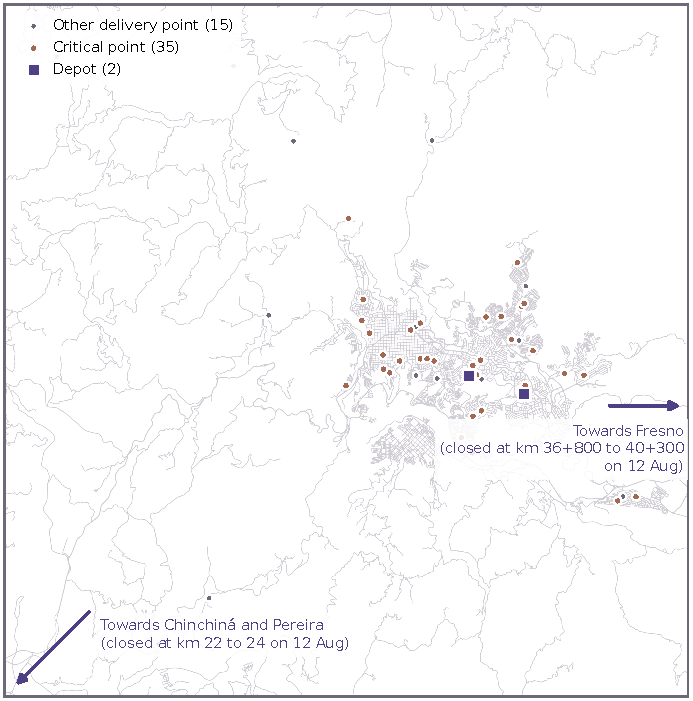
\includegraphics[width=0.62\linewidth]{figuras/map_manizales.pdf}
\caption{Road network of Manizales and Villamaría (grey), with the 50 delivery points and the two depots of the public scenario. Arrows show the direction of the two corridors that remained fully closed on 12 August 2026; the closures themselves lie outside the frame \citep{semana2026vias}. Road data \copyright{} OpenStreetMap contributors, available under the Open Database Licence. Generated by \code{figuras/scripts/map\_manizales\_en.py}.}
\label{fig:map}
\end{figure}

\begin{table}[ht]
\centering
\small
\caption{Data used by DespachoX and its simulation. ``Sourced'' means taken from a public source with a link per row; ``synthetic'' means generated by the team; ``assumed'' means a value chosen by the team without a source. No source in this table has yet been opened by a member of the team.}
\label{tab:data}
\begin{tabularx}{\linewidth}{L{3.3cm} Y L{2.6cm}}
\toprule
Dataset & Content & Status \\
\midrule
Road network & OpenStreetMap drivable network of Manizales and Villamaría plus the access roads to La Siria, Neira, Letras and the Autopista del Café; 7,825 nodes after keeping the largest strongly connected component \citep{boeing2017osmnx} & Sourced \\
Delivery points & 50 points with source and coordinates, 35 of them critical (shelters, child development centres, hospitals, care homes), across the 12 urban districts and rural areas & Sourced \\
Depots & Banco de Alimentos de Manizales and the Coliseo Menor collection centre; cold storage unknown & Sourced; cold storage unknown \\
Reference fleet & 9 vehicles: 3 trucks (5,115, 2,000 and 2,000\,kg), 4 light vehicles (three 4$\times$4 pick-ups of 845\,kg and a van of 800\,kg) and 2 motorcycles (40\,kg); capacities from manufacturer sheets and public tenders & Sourced as reference; not the real fleet of Manizales \\
Rations & 555\,g of dry ration per person per day, summed by the team from the UNHCR column of a comparative ration table \citep{logcluster_commodities}; 2.9 persons per household in Manizales \citep{dane2019manizales} & Sourced; the sum is ours \\
Shelf life & Hours without and with refrigeration per product, from ICBF, FDA, USDA and FAO documents & Sourced; some values assumed \\
Closure records & 178 records: 23 after the earthquake, one standing restriction and 154 antecedents from 2017 to 2026, from registry \#767 and the press \citep{invias767} & Sourced \\
Place names & 452 names and aliases of neighbourhoods, roads and sites; aliases written by the team & Sourced and assumed \\
Orders and lots & Requests and inventory for demonstration and testing & Synthetic \\
\bottomrule
\end{tabularx}
\end{table}
% Files: datos_publicos/*.csv with *_fuentes.csv; docs/datos/*.md; despliegue/grafo/manizales_region.graphml; lugares/.
% CODE-vs-DOC: persons per family is 4 in entrada/raciones.py (assumption, no source) and 2.9 in the public
% scenario (DANE 2018); kg per family is 10 in despacho/optimizar.py and 12 in despacho/sim/escenario.py.

% ======================================================================================
\section{System design}\label{sec:system}

\subsection{Design principle: read, compute, decide}

The architecture rule gives each kind of work to the component suited to it and keeps accountability with people. A language model reads messages and structures them into records with a fixed schema. It never assigns a vehicle, chooses a route or dispatches anything. Deterministic code and an optimizer compute plans from those records, from the stock and from the confirmed state of the roads. A human dispatcher decides, and every state change that moves food passes through a person. The rule comes from CARMEN, project 56031 funded by Minciencias, where the same division of work was applied \citep{PORVERIFICAR_carmen}. % VERIFY with Carlos: how to cite CARMEN, and whether to name it at all before authorship is settled.

The rule answers two concerns. The first is reliability. Language models fail more often on urgent requests and on messages with typing errors \citep{imran2025robustness}, which are the messages a relief desk most needs to read correctly. Accountability is the second. A dispatcher who approves a plan answers for it, and the log shows who approved what and when.

Three gates enforce the rule in the data model (Figure~\ref{fig:flow}). An order stays \code{nuevo} until a dispatcher confirms it, and it cannot be confirmed without a confirmed location. A road closure stays \code{reportado} until a dispatcher confirms it, and only confirmed closures alter the road network. A plan is born \code{propuesto} and becomes \code{aprobado} only when a named dispatcher approves it. Packages and their codes are created at that moment. Every confirmation, approval and delivery is written to a log with the name of whoever made it.

\begin{figure}[ht]
\centering
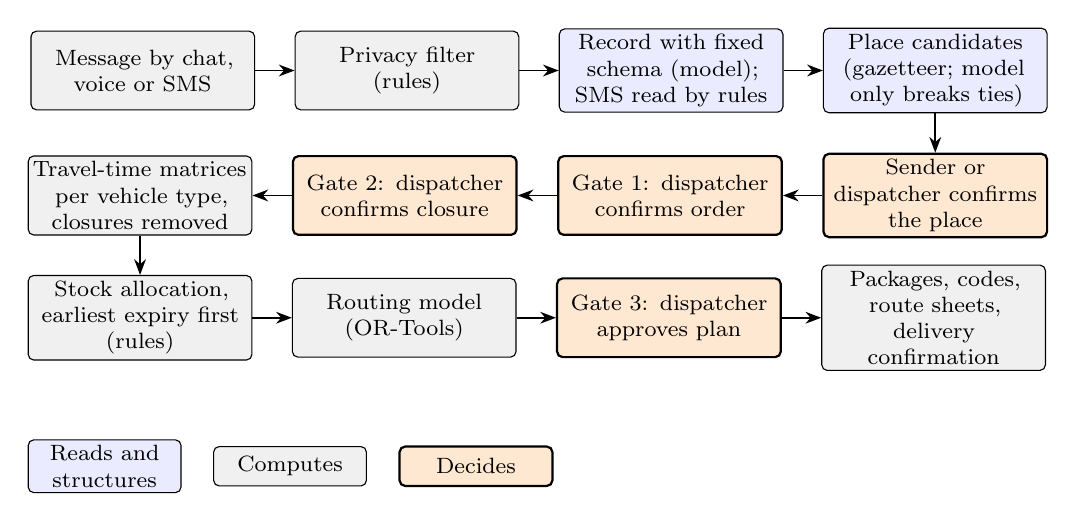
\begin{tikzpicture}[
  node distance=5mm and 5mm,
  box/.style={draw, rounded corners=2pt, align=center, font=\footnotesize, minimum height=10mm, text width=27mm, inner sep=2pt, execute at begin node={\hyphenpenalty=10000\exhyphenpenalty=10000\relax}},
  model/.style={box, fill=blue!8},
  rule/.style={box, fill=gray!12},
  human/.style={box, fill=orange!18, thick},
  arr/.style={-{Stealth[length=2mm]}, semithick}
]
\node[rule]  (msg)  {Message by chat,\\ voice or SMS};
\node[rule,  right=of msg]  (priv) {Privacy filter\\ (rules)};
\node[model, right=of priv] (ext)  {Record with fixed\\ schema (model);\\ SMS read by rules};
\node[model, right=of ext]  (loc)  {Place candidates\\ (gazetteer; model\\ only breaks ties)};
\node[human, below=of loc]  (g0)   {Sender or\\ dispatcher confirms\\ the place};
\node[human, left=of g0]    (g1)   {Gate 1: dispatcher\\ confirms order};
\node[human, left=of g1]    (g2)   {Gate 2: dispatcher\\ confirms closure};
\node[rule,  left=of g2]    (mat)  {Travel-time matrices\\ per vehicle type,\\ closures removed};
\node[rule,  below=of mat]  (alloc){Stock allocation,\\ earliest expiry first\\ (rules)};
\node[rule,  right=of alloc](route){Routing model\\ (OR-Tools)};
\node[human, right=of route](g3)   {Gate 3: dispatcher\\ approves plan};
\node[rule,  right=of g3]   (pkg)  {Packages, codes,\\ route sheets,\\ delivery confirmation};
\draw[arr] (msg) -- (priv);
\draw[arr] (priv) -- (ext);
\draw[arr] (ext) -- (loc);
\draw[arr] (loc) -- (g0);
\draw[arr] (g0) -- (g1);
\draw[arr] (g1) -- (g2);
\draw[arr] (g2) -- (mat);
\draw[arr] (mat) -- (alloc);
\draw[arr] (alloc) -- (route);
\draw[arr] (route) -- (g3);
\draw[arr] (g3) -- (pkg);
\node[model, minimum height=5mm, text width=18mm, below=10mm of alloc.south west, anchor=north west] (lm) {Reads and structures};
\node[rule,  minimum height=5mm, text width=18mm, right=4mm of lm] (lr) {Computes};
\node[human, minimum height=5mm, text width=18mm, right=4mm of lr] (lh) {Decides};
\end{tikzpicture}
\caption{Data flow of DespachoX. Colours mark which component acts at each step. Gate 1 applies to orders and Gate 2 to closure reports, which follow the same intake path. A rejected plan leaves the last approved plan in force.}
\label{fig:flow}
\end{figure}

\subsection{Intake of requests and road reports}

Requests and road reports enter through a Telegram bot. Before anything else, a privacy filter removes what looks like telephone numbers, identity numbers, e-mail addresses and names introduced by formulas such as \emph{me llamo} (my name is). The filter is a heuristic, and it can miss personal data written in unexpected forms. It runs before the text reaches the language model and before anything is stored. The sender is stored as a salted keyed hash of the chat identifier, so the system can answer status queries without keeping the identifier.

A hosted language model then reads the cleaned text and returns a record that must validate against a strict schema: an order, a closure, both, or neither. % Model in code: claude-haiku-5-5 via the Anthropic API (entrada/extraer.py).
The instructions tell the model to copy what the message says and to leave empty what it does not say. In particular, it must not complete quantities or guess places. Conversions of persons and infants into families and kilograms happen in the code, under written rules. When the model fails or returns an invalid record, the same text goes to the rule-based SMS reader, and if that also fails the message is stored as raw text for the dispatcher. No message is discarded. Voice notes are transcribed by an external service when one is configured, and the audio is not stored.

We measured the extractor on fifteen synthetic messages written by the team, with misspellings, abbreviations and mixed orders and closures. It returned 62 of 64 fields correctly (96.9\%) in one run, at about 1.8\,s per message. The messages were written by the same team that wrote the instructions, so the figure serves as a regression check. Accuracy on real messages remains unmeasured.

\subsection{Locations, duplicates and silent points}

A request is useful only if its place is known, and residents name places in their own way. A gazetteer of 452 names and aliases of neighbourhoods, roads and sites resolves the place in steps: exact match, then approximate match tolerant to typing errors, then, if several candidates remain, a language model that may only pick one of the listed candidates or answer that none fits. If nothing fits, the bot asks for a map pin or a nearby neighbourhood, and the dispatcher can also move the pin on the map. The resolved place is sent back to the sender, and only a confirmation by the sender or by the dispatcher writes it into the order. Confirmed phrasings become new aliases. On 44 test phrases written by the team, without the model, the resolver proposed the correct place with confidence 30 times, listed it among options 5 times, and answered that it did not know 9 times; all 9 named places absent from the gazetteer. It never proposed a wrong place with confidence. The phrases were written by people who knew the gazetteer, so the test protects against regressions and says little about real messages.

Two rules deal with what is repeated or missing. A second order from the same point within two hours is linked to the first as a duplicate and is not counted twice. A critical point that has gone six hours without an order with a confirmed location generates a silence alert, which enters the dispatcher's queue as a verification visit. A silence alert never leaves the warehouse with food, even if confirmed.

A separate rule-based module, not yet connected to the bot, filters suspicious requests, with spatio-temporal clustering, a Poisson test for bursts and a Bayesian score whose parameters are declared assumptions. It has been tested on ten synthetic scenarios, and only a person can confirm or discard a request it flags.

\subsection{Road closures and re-planning}

Drivers and rescuers report closures in the same chat, and the record lists which vehicle types cannot pass. A closure is placed on the road graph through a list of 15 named road segments, or else on the nearest edge within 500\,m of the reported coordinates. A closure whose location still awaits confirmation is not applied, and none enters the plan before a dispatcher confirms it. A confirmed closure removes the edge in both directions for the vehicle types it blocks, and the optimizer then solves the problem again. Loads already on board a vehicle in transit stay with that vehicle, and the vehicle starts from its current position. The last approved plan remains in force until the dispatcher approves the new one.

\subsection{Traceability}

When a plan is approved, each stop receives a package with a four-character code drawn from an alphabet of 25 characters that cannot be confused when dictated, which gives 390,625 possible codes. The printed route sheet carries one QR code per package and a map drawn without internet access. Whoever receives the package, or the driver, confirms delivery by sending the word for ``delivered'' and the code by Telegram or SMS, and the package and its order are closed in the log. A person who guesses a code can mark someone else's package as delivered. The pilot will accept a confirmation only from the destination or from the assigned driver.

\subsection{Operation without connectivity}

The system degrades in steps when connectivity fails. Requests, closures and delivery confirmations can arrive as short SMS with a fixed format, for example \code{PEDIDO 40 SAN JOSE ARROZ LECHE}, which a rule-based reader parses without a model or a network. The reader tolerates typing errors in keywords, variable word order and filler words, and it answers within 160 characters without accents so that the reply fits a single message. It read 20 of 20 synthetic messages correctly, in a test that is not independent because the same session wrote the cases and the rules. An Android phone in the warehouse runs an open-source SMS gateway and forwards each message to the dispatch laptop over local Wi-Fi. That path has been tested with a simulated phone; a test with a real phone is pending. 

The optimizer, the road network and the gazetteer also run on a laptop without internet access. With network access blocked in software, the system went from loading data to a printed route sheet and a recorded delivery in 23\,s; the test has not been repeated with Wi-Fi switched off. The dashboard map still needs internet access to load its libraries.

\subsection{Scale and cost}

Message intake was load-tested with a simulated extractor that reproduces the latency of the real model. Five thousand messages arriving at once were processed at 914 per minute, with none lost. In a run of 1,000 messages with 5\% of readings forced to fail, the 59 affected messages were stored as raw text for the dispatcher. The bottleneck is the place resolver, which compares each text with every name in the gazetteer. The cost of reading messages with the hosted model is an estimate, between 1.75 and 4.50\,USD per 10,000 messages, from public prices and assumed token counts; it has not been measured with the real model.

% ======================================================================================
\section{Optimization model}\label{sec:model}

The optimizer in \code{despacho/optimizar.py} builds a routing model and hands it to the OR-Tools routing library \citep{ortools_routing}, with travel times from \code{despacho/matriz.py} and \code{despacho/red.py}. Where the code and the team's documentation disagree, the statement follows the code and records the disagreement. The solver is a heuristic. It returns the best plan found within a time limit and offers no optimality guarantee.

\subsection{Road network and travel times}

The road network is a directed multigraph $G=(N,E)$ built from OpenStreetMap with OSMnx \citep{boeing2017osmnx}. Each edge $e$ has a length and a speed, taken from its \code{maxspeed} tag when present and otherwise from a default per road class (Table~\ref{tab:params}). Its base travel time $\tau_e$ is length divided by speed. Each vehicle type $m\in\mathcal{M}=\{\text{truck},\text{4}{\times}\text{4},\text{motorcycle}\}$ sees its own subnetwork. Trucks may not use residential, living-street, service, track, path or pedestrian edges, nor edges tagged as closed to heavy goods vehicles or with a weight limit below 5\,t. The 4$\times$4 and the motorcycle use the whole drivable network. A type factor $\phi_m$ scales travel times, with $\phi_{\text{truck}}=1.25$, $\phi_{4\times4}=1.0$ and $\phi_{\text{moto}}=0.9$. A confirmed closure removes its edge in both directions from the subnetworks of the types it blocks.

Each depot, delivery point and vehicle in transit is attached to the nearest node of the subnetwork of each type. The attachment ignores closures, so a place cut off by a closure becomes unreachable and keeps its location. A place farther than 300\,m from the truck network, or 400\,m from the network of the other types, is unreachable for that type; a truck may park within 300\,m of a point and unload by hand. Shortest-path times $t^m_{ab}$ between all pairs of places, over edge times $\phi_m\tau_e$, are computed with Dijkstra's algorithm, rounded to integer seconds, and set to $10^7$\,s when no path exists.

\subsection{Rule-based preparation}

Several decisions are made by rules before the solver runs, and the solver cannot revise them. % CODE-vs-DOC: docs (FICHA, ESTADO_DEL_ARTE) describe "prioridad a lo que vence primero" as part of the optimizer; in code, stock allocation is a greedy rule applied before routing, so allocation and routing are sequential, unlike the joint model of Balcik et al. (2008).

\paragraph{Admitted orders.} The model considers orders in state \code{confirmado}, with a confirmed delivery point, not marked as duplicates and not generated by a silence alert. When the dispatcher asks for a re-plan, orders already assigned in the approved plan are planned again, except those on board a vehicle in transit, which stay with that vehicle. In an ordinary plan, the allocation rule first reserves stock for the orders already assigned, and new orders draw on what remains.

\paragraph{Demand lines.} Each order becomes a list of product lines in kilograms. A line without a stated quantity receives a share of the order's estimated total, which defaults to 10\,kg per family; an order with neither kilograms nor families is treated as one family. A line without a named product is a generic food package that only non-perishable lots can serve. Every quantity completed by these rules is flagged in the plan so that the dispatcher can confirm it with the requester.

\paragraph{Effective expiry.} Let $t_0$ be the planning time and $e_l$ the expiry of lot $l$. The model uses an effective expiry $\hat e_l = t_0 + \psi_l\,(e_l - t_0)$ for $e_l>t_0$, and $\hat e_l=e_l$ otherwise. The factor is $\psi_l=1.2$ for perishable fruit in active packaging that captures ethylene, stored in a depot with cold storage, and $\psi_l=1$ for every other lot. The value 1.2 is a lower bound that the team derived from one fruit, purple passion fruit stored at 8\,°C, in the patent application of the packaging \citep{PORVERIFICAR_patente37476}; no other product has been tested, and the plan declares the factor as an assumption.

\paragraph{Stock allocation.} Orders are processed by decreasing urgency, then by earliest deadline, then by identifier. For each order the rule considers every depot that has a free vehicle able to reach the point and return. For each such depot it allocates lots greedily, line by line, in increasing order of effective expiry. It skips a perishable lot whose effective expiry falls at or before $t_0+\theta_{ai}+\mu$, where $\theta_{ai}$ is the fastest travel time from depot $a$ to the point of order $i$ among that depot's candidate vehicles and $\mu=1{,}800$\,s is a safety margin. The order is assigned to the depot that covers the most kilograms, with ties broken by shorter travel time, and the allocation is committed before the next order is processed. An order that no vehicle can reach, that no stock covers, or that fits in no vehicle able to reach it is reported as unserved with its reason and does not enter the solver.

\subsection{Sets, parameters and variables}

Let $\mathcal{K}$ be the set of usable vehicles: those of a modelled type, assigned to a depot and not out of service. % CODE-vs-DOC: the schema allows vehicle type a_pie (on foot), but the optimizer only models camion, campero and moto; other types are left out with a warning. Drones and animal traction, named in the challenge, are not modelled.
Vehicle $k$ has type $m(k)$, capacity $Q_k$ in grams, a start node $o_k$ and an end node $d_k$. The start node is its depot if the vehicle is free and its current position if it is in transit; the end node is always its depot. Drones and animal traction, which the challenge lists, are not modelled, and neither are deliveries on foot, which the data schema allows. Let $\mathcal{P}$ be the set of orders that passed the preparation. Each order $i\in\mathcal{P}$ is a node located at its delivery point and has:
\begin{itemize}
\item an allocated load $q_i$ in grams and a perishable mass $w_i$ in kilograms;
\item an urgency $u_i\in\{1,2,3\}$, where 3 is the most urgent;
\item a criticality factor $c_i=\gamma=3$ if its point is critical and $c_i=1$ otherwise;
\item a soft due time $b_i=\max(0,\ell_i-t_0)$ in seconds, where $\ell_i$ is the deadline stated in the order or, if none, its creation time plus $L(u_i)$, with $L(3)=4$\,h, $L(2)=12$\,h and $L(1)=24$\,h;
\item if it carries perishables, a hard due time $h_i=(\hat e_i - t_0)-\mu$, where $\hat e_i$ is the earliest effective expiry among the perishable lots allocated to it;
\item a set $\mathcal{K}_i\subseteq\mathcal{K}$ of allowed vehicles: those based at the depot chosen for $i$, with $Q_k\geq q_i$, which either carry $i$ already or are free and can reach the point of $i$ and return to their depot.
\end{itemize}
The service time is $s_i=600$\,s at every order node and $s_a=0$ at start and end nodes. The horizon is $H=86{,}400$\,s. The lateness weight is $\alpha_i=\beta(u_i)\,c_i$ per second, with $\beta(1)=1$, $\beta(2)=3$ and $\beta(3)=10$. The penalty for leaving order $i$ unserved is
\begin{equation}
\pi_i = 2\times 10^{7}\,u_i\,c_i + \left\lfloor 2\times 10^{4}\,w_i \right\rfloor .
\end{equation}
The decision variables are $x^k_{ab}\in\{0,1\}$, equal to 1 if vehicle $k$ travels directly from node $a$ to node $b$; $z_i\in\{0,1\}$, equal to 1 if order $i$ is left unserved; the arrival time $T_a\geq 0$ at node $a$, in seconds after $t_0$; and the load $Y_a\geq 0$ accumulated on arrival at node $a$.

\subsection{Objective and constraints}

The model minimizes
\begin{equation}\label{eq:obj}
\sum_{k\in\mathcal{K}}\sum_{a,b} \bigl(t^{m(k)}_{ab}+s_a\bigr)\,x^k_{ab}
\;+\;\sum_{i\in\mathcal{P}} \alpha_i \,\max\bigl(0,\;T_i-b_i\bigr)
\;+\;\sum_{i\in\mathcal{P}} \pi_i\, z_i ,
\end{equation}
subject to
\begin{align}
&\sum_{k\in\mathcal{K}}\sum_{a} x^k_{ai} + z_i = 1 && \forall i\in\mathcal{P}, \label{eq:once}\\
&x^k_{ai} = 0 && \forall i\in\mathcal{P},\ k\notin\mathcal{K}_i,\ \forall a, \label{eq:allowed}\\
&\textstyle\sum_{b} x^k_{o_k b} = 1,\quad \sum_{a} x^k_{a d_k} = 1,\quad \sum_a x^k_{ai}=\sum_b x^k_{ib} && \forall k\in\mathcal{K},\ i\in\mathcal{P}, \label{eq:flow}\\
&x^k_{ab}=1 \;\Rightarrow\; T_b = T_a + s_a + t^{m(k)}_{ab} && \forall k,a,b, \label{eq:time}\\
&T_{o_k}=0,\qquad 0\leq T_a\leq H && \forall k,a, \label{eq:horizon}\\
&T_i \leq \min\bigl(H,\max(0,h_i)\bigr) && \forall i\in\mathcal{P}\text{ with perishables}, \label{eq:expiry}\\
&x^k_{ab}=1 \;\Rightarrow\; Y_b = Y_a + q_a,\qquad Y_{o_k}=0,\qquad Y_a\leq Q_k && \forall k,a,b, \label{eq:load}
\end{align}
with $q_a=0$ at start and end nodes. Constraint~\eqref{eq:once} serves each order at most once or leaves it unserved at its penalty. Constraint~\eqref{eq:allowed} restricts each order to its allowed vehicles. Constraints~\eqref{eq:flow} give each vehicle a single route from its start to its depot, possibly empty. Constraint~\eqref{eq:time} propagates time with no waiting, which is harmless because no order has an earliest delivery time. Constraint~\eqref{eq:expiry} is the hard expiry deadline of perishables, measured on arrival at the point, before unloading. Constraint~\eqref{eq:load} keeps every load within capacity.

The three terms of the objective differ by orders of magnitude. The smallest penalty for an unserved order, $2\times10^{7}$, equals about 231 days of travel time. A second of lateness costs between 1 and 30 units, so the lateness of one order over the whole horizon costs at most $30\times 86{,}400\approx 2.6\times10^{6}$. The objective therefore favours serving every order that fits within the horizon, the capacities and the expiry deadlines. Whether the heuristic search finds such a plan is a separate matter. Among served orders, a second of lateness of a critical order of urgency~3 weighs thirty times a second of travel. The objective is a surrogate for the social cost advocated by \citet{holguinveras2013objective}, and its weights are our assumptions.

Three features of the implementation shape the plans. % CODE-vs-DOC: the docstring of optimizar.py says the objective is travel time + weighted lateness + penalties; the arc cost also includes the service time of the origin node (600 s per served order), as in Eq. (2).
First, the arc cost includes the service time of its origin node, so each served order adds 600\,s to the objective; against the penalties this is negligible. Second, each vehicle performs a single trip. A vehicle that returns to its depot receives new orders only in a later plan. Third, every order at the same point is a separate node, with its own service time.

\subsection{Search}

The solver builds a first solution with the path-cheapest-arc strategy and improves it with guided local search, which the OR-Tools documentation describes as generally the most efficient metaheuristic for vehicle routing \citep{ortools_routing_options}. The search stops at a time limit, 8\,s by default in the product and never more than 10\,s; the simulation uses 1\,s per call. On the demonstration instance of 17 orders, with 3\,s of search, a plan took between 3.4 and 3.8\,s. On the public scenario built from the data of Table~\ref{tab:data}, with 25 confirmed orders and 3\,s of search, the plan served all 25 orders and reached all 23 critical stops before their deadlines, in 3.5\,s. The punctuality figures are the plan's own estimates of arrival under the assumed speeds of Table~\ref{tab:params}, which are under revision. Because the search stops on wall-clock time, two runs on the same input can return slightly different plans.

\begin{table}[ht]
\centering
\small
\caption{Parameters of the optimization model as set in the code, with their status. ``Assumed'' means chosen by the team without a source.}
\label{tab:params}
\begin{tabularx}{\linewidth}{L{5.2cm} L{4.2cm} Y}
\toprule
Parameter & Value in code & Status \\
\midrule
Default speed by road class (km/h) & trunk 50, primary 40, secondary 35, tertiary 30, unclassified 25, residential 20 & Assumed; OSM \code{maxspeed} used when present \\
Speeds of a diesel bus in Manizales, by road class and slope (not in the optimizer) & 21.8 to 24.2 on main roads; 16.2 to 17.5 on collector roads; 22.6 on average & Sourced, Table~14 of \citet{ocampo2019costos}; copied to \code{datos\_publicos/}\allowbreak\code{velocidades.csv} to replace the defaults \pend{[SIM-CONFIG]} \\
Vehicle time factor $\phi_m$ & truck 1.25, 4$\times$4 1.0, motorcycle 0.9 & Assumed \\
Snapping tolerance & truck 300\,m, others 400\,m & Assumed \\
Service time $s_i$ & 600\,s per stop & Assumed \\
Expiry margin $\mu$ & 1,800\,s & Assumed \\
Default deadline $L(u)$ & 4, 12 and 24\,h for urgency 3, 2 and 1 & Assumed \\
Lateness weight $\beta(u)$ & 10, 3 and 1 per second & Assumed \\
Criticality factor $\gamma$ & 3 & Assumed; chosen after an exploratory sweep \\
Unserved penalty & $2\times10^{7}\,u_i c_i$ plus $2\times10^{4}$ per perishable kg & Assumed \\
Packaging factor $\psi$ & 1.2 for packed fruit in cold storage & Lower bound derived from one patent figure \\
Default mass per family & 10\,kg & Assumed \\
Search limit & 8\,s (product), 1\,s (simulation), at most 10\,s & Chosen \\
\bottomrule
\end{tabularx}
\end{table}
% The value gamma = 3 was adopted after a sweep of 1, 3, 10 and 30 that did not satisfy the selection rule written before
% that sweep (docs/SIMULACION.md, 8.1-8.3). Say so in the final paper, and make sure the evaluation seeds of the
% reported run are disjoint from the sweep seeds (20261120-20261149) and the confirmation seeds (20261150-20261179).
% [SIM-CONFIG]

% ======================================================================================
\section{Simulation design}\label{sec:simdesign}

The simulation estimates how much the dispatch policy alone changes the two indicators of the challenge. Each policy dispatches the same synthetic day, with the same orders, stock, fleet and closures, so that differences between policies are paired by construction. The code is in \code{despacho/sim/} and calls the same optimizer as the product, with the same road network; a test fails if the travel-time matrices of the simulation and of the optimizer differ by more than one second.

\subsection{Scenarios}

Each random seed generates one day of operation. Table~\ref{tab:simparams} lists the generator's parameters. In brief, between 30 and 80 delivery points are drawn among network nodes within 6\,km of the city centre, at least 250\,m apart and reachable by a 4$\times$4 vehicle in both directions, and 20\% of them are critical. A single depot sits on the truck-accessible node nearest to the main square. Orders arrive during the first 8 hours, 40\% of them already queued at the start. Perishable stock equals perishable demand and comes in lots that expire between 6 and 48 hours after the start, while non-perishable stock is unlimited. The fleet scales with the number of points. Between three and eight road segments close during the day, in both directions. They are drawn among the edges used by shortest paths from the depot to the points, with probability proportional to the number of such paths, because a closure on a street that no vehicle uses tests no policy. As a consequence, simulated closures disrupt more than closures drawn uniformly over the network.

\begin{table}[ht]
\centering
\small
\caption{Parameters of the scenario generator (\code{despacho/sim/escenario.py}). All values are assumptions of the team except the road network. Rows marked \pend{[SIM-CONFIG]} may change in the reported run.}
\label{tab:simparams}
\begin{tabularx}{\linewidth}{L{4.6cm} Y}
\toprule
Element & Value \\
\midrule
Delivery points & Uniform integer in [30, 80]; within 6\,km of the centre; at least 250\,m apart; 20\% critical \\
Orders per day & $\max\bigl(P/2,\ \mathrm{Poisson}(\lambda P)\bigr)$ for $P$ points, with $\lambda=2$, 2.5 or 3 orders per point (light, medium and high load) \\
Arrival of orders & 40\% at time 0; the rest uniform over the first 8\,h \\
Size of an order & Uniform integer between 3 and 50 families; 12\,kg per family; perishable share uniform in [0.2, 0.5] \\
Urgency & Critical points: 3 with probability 0.8, otherwise 2. Other points: 1, 2 or 3 with probabilities 0.4, 0.5 and 0.1 \\
Deadline after creation & 3, 5 and 8\,h for urgency 3, 2 and 1 \\
Perishable stock & Equal to perishable demand, in lots of 100 to 400\,kg expiring uniformly between 6 and 48\,h \pend{[SIM-CONFIG]} \\
Non-perishable stock & Unlimited \\
Fleet & One truck of 3,000\,kg per 30 points, one 4$\times$4 of 700\,kg per 15 points, one motorcycle of 60\,kg per 20 points; at least one of each \\
Closures & Uniform integer in [3, 8] per day; 30\% present at time 0 and unknown; the rest uniform over the first 8\,h; never lifted; block trucks always, 4$\times$4 with probability 0.7, motorcycles with probability 0.3; none within 400\,m of the depot \\
Loading and unloading & 10\,min per trip at the depot; 10\,min per delivery \\
Discovery of a closure & A vehicle that reaches an unknown closure loses 3\,min, reports it and detours; all vehicles heading there are diverted \\
Human delays & Closure confirmed 5\,min after the report; each plan approved in 2\,min, one plan at a time \\
Re-planning batch & Every 30\,min \\
Day length & 14\,h; whatever is not delivered by then counts as undelivered \\
Road network & Urban network of Manizales and Villamaría, or the extended network with access roads \pend{[SIM-CONFIG]} \\
Travel speeds & As in the optimizer \pend{[SIM-CONFIG]: bus speeds of Table~\ref{tab:params} or defaults} \\
Optimizer search & 1\,s per call; criticality factor $\gamma=3$ \pend{[SIM-CONFIG]} \\
Language model & Assumed error-free in reading orders and closures \\
\bottomrule
\end{tabularx}
\end{table}
% [SIM-CONFIG] Check against the run of 21 Nov 2026: speed table (datos_publicos/velocidades.csv?), shelf-life rule for
% lots, FACTOR_CRITICO, network file (manizales.graphml or manizales_region.graphml), seeds, number of seeds per load.

\subsection{Engine and information}

The engine is a discrete-event simulator. Vehicles advance edge by edge on the true network, while paths are computed on the known network, which lacks the closures that nobody has reported yet. The engine enforces three rules on every policy. No vehicle carries more than its capacity. A perishable kilogram that arrives after its lot expires does not count as delivered. An unknown closure changes no route. Two further rules handle vehicles trapped by closures. A vehicle with no way back on its own subnetwork may return over any drivable road at twice the travel time. A vehicle with no way back at all leaves service, its load is lost and its orders return to the queue.

\subsection{Policies}

Four policies dispatch the same days (Table~\ref{tab:policies}). The naive policy is what a dispatcher with a spreadsheet and a phone might do without priorities. The expert policy adds the two rules of an experienced dispatcher, urgency first and earliest expiry first, and it is the demanding baseline, for the reasons given in Section~\ref{sec:related}. Planning once and never again isolates the value of re-planning, with one confound. Orders that arrive after the initial plan are served with the naive rule, so the comparison mixes re-planning with prioritizing new orders.

\begin{table}[ht]
\centering
\small
\caption{Dispatch policies compared in the simulation.}
\label{tab:policies}
\begin{tabularx}{\linewidth}{L{3.3cm} Y}
\toprule
Policy & Behaviour \\
\midrule
\code{ingenua} (naive) & Serves orders by arrival. Gives the oldest order the free vehicle that reaches it fastest and fills that vehicle with the next orders in the queue that fit. The driver sequences stops by nearest neighbour. Lots leave the warehouse in order of entry. Detours only on meeting a closure. \\
\code{experta} (expert) & The naive policy with two rules: urgent orders first, and the earliest-expiring lots first. \\
\code{optimiza\_una\_vez} & The optimizer plans once at the start; later orders are served with the naive rule. \\
\code{despachox} & The optimizer plans at the start and again at each confirmed closure, at each 30-minute batch of orders and whenever a vehicle returns to the depot. \\
\bottomrule
\end{tabularx}
\end{table}

The baselines receive several advantages. They decide instantly, while each optimized plan waits two minutes for approval and only one plan is reviewed at a time. They see each order the moment it arrives, while \code{despachox} sees it at the next batch or when a vehicle returns. Their drivers receive every closure notice that DespachoX drivers receive. The cap on stops per trip of the naive rule was calibrated in its favour on calibration seeds distinct from the evaluation seeds, and the best setting was no cap. % CODE-vs-DOC: in the product, re-planning is triggered by a confirmed closure or by the dispatcher (despacho/recalcular.py); the periodic triggers (30-min batches, vehicle returns) belong to the simulated policy.

\subsection{Load levels, seeds and statistics}

Three load levels, of 2, 2.5 and 3 orders per point and day, span conditions from slack to stress. They were chosen on calibration seeds 100 to 111 by looking only at the naive policy, so that it is neither idle nor collapsed; with lower demand every policy delivers almost everything on time and the comparison loses its power. Each load level is run with \pend{[SIM]} seeds, the same for all policies. % [SIM-CONFIG] seed range of the reported run.
For each metric and pair of policies we report the mean paired difference across seeds with a 95\% confidence interval from Student's $t$ distribution, and the number of seeds in which each policy wins, ties or loses. The two indicators of the challenge are the primary outcomes: the share of orders from critical points delivered by their deadline, and the share of perishable kilograms that expire undelivered. All other metrics are secondary. We do not adjust intervals for multiple comparisons, so secondary differences should be read as descriptive. % PROPOSAL for Carlos: primary/secondary split and no multiplicity adjustment are our framing; the code reports all metrics alike.

\subsection{Metrics}

The simulation computes fourteen metrics per seed and policy (\code{despacho/sim/metricas.py}):
\begin{enumerate}[label=M\arabic*.]
\item Orders from critical points delivered by their deadline (\%). Undelivered orders count as late.
\item Perishable kilograms expired without delivery (\%), over all perishable kilograms in stock, including what expired in the warehouse, on board or on arrival.
\item Orders delivered by their deadline, all points (\%).
\item Orders delivered within the day (\%).
\item Requested kilograms that did not arrive in good condition (\%).
\item Mean time from order to delivery (h).
\item Maximum time from order to delivery (h).
\item Mean waiting time at the worst-served point (h), where undelivered orders wait until the end of the day.
\item Kilometres driven by the fleet.
\item Vehicles left without any path back by a closure.
\item Returns to the depot over roads not suited to the vehicle.
\item Arrivals at a wrong point caused by registration errors (variant with location errors only).
\item Calls to the optimizer.
\item Mean and maximum solve time per call (s).
\end{enumerate}

\subsection{Sensitivity analyses}

The code supports variants that probe the main assumptions. With probability $p$ an order is registered at a wrong point; without location confirmation the error is discovered when a vehicle arrives there, and with confirmation it is corrected before dispatch at the cost of five minutes. Other variants fix the number of closures, remove 4$\times$4 vehicles from the fleet, change the search time per call, change the criticality factor or use the extended network with the access roads. Which variants are reported is \pend{[SIM]}. The location-error rate has no source, so any result that depends on it inherits that weakness.

\subsection{Known sources of optimism and pessimism}

Several assumptions favour every policy. Every reported closure is real, confirmed in five minutes and never lifted. The dispatcher approves every plan in two minutes, and drivers follow every plan. There is one depot and one day, without restocking, and travel times are deterministic. One assumption favours DespachoX alone. The language model reads every order and closure correctly, and only DespachoX depends on it. Two choices work in the opposite direction. Closures fall on the roads that vehicles use, so they disrupt more than random closures would, and one second of search per call is short compared with the eight seconds of the product. Finally, the search stops on wall-clock time, so repeating a run with the same seeds gives slightly different figures.

% ======================================================================================
\section{Results}\label{sec:results}

% How to fill: despacho/sim/correr.py writes resultados.csv and resumen.md in the output folder of the run.
% Fast path: nice -n 19 /home/claude/venv-dx/bin/python -I docs/manuscrito/llenar_resultados.py <run>/resultados.csv \
%   --commit <hash> > docs/manuscrito/resultados_tablas.tex ; then replace Tables tab:scen, tab:means and tab:diff
%   below by \input{resultados_tablas}. The script mirrors correr.py (tested on the first-round CSV in /tmp, not kept).
% Table tab:scen <- the line "Escenarios: ..." of each load level in resumen.md.
% Table tab:means <- "Media por política (desviación estándar entre semillas)" of each load level.
% Table tab:diff <- the paired differences with IC 95 % and the win/tie/loss counts.
% All cells below are filled from the run of 21 November 2026 (expected ~6 a.m.), copied without change from its
% summary file, with the commit hash of the code that produced them. Report them as they came out, with the
% baseline, the number of scenarios and the assumptions. Do not round to make a policy look better.

The run reported here used commit \pend{[SIM]} of the repository, \pend{[SIM]} seeds per load level and \pend{[SIM]} simulated days in total. \pend{[SIM]} calls to the optimizer ended in error. Table~\ref{tab:scen} describes the scenarios, Table~\ref{tab:means} gives the mean of each metric by policy and Table~\ref{tab:diff} the paired differences.

\begin{table}[ht]
\centering
\small
\caption{Scenarios by load level: means across seeds.}
\label{tab:scen}
\begin{tabular}{lccc}
\toprule
 & Light & Medium & High \\
\midrule
Delivery points (critical) & [SIM] & [SIM] & [SIM] \\
Orders & [SIM] & [SIM] & [SIM] \\
Requested mass (t) & [SIM] & [SIM] & [SIM] \\
Vehicles & [SIM] & [SIM] & [SIM] \\
Closures (discovered) & [SIM] & [SIM] & [SIM] \\
\bottomrule
\end{tabular}
\end{table}

\begin{table}[ht]
\centering
\small
\caption{Mean (standard deviation across seeds) of each metric by policy and load level. M1 and M2 are the primary outcomes.}
\label{tab:means}
\begin{tabular}{llcccc}
\toprule
Load & Metric & \code{ingenua} & \code{experta} & \code{optimiza\_una\_vez} & \code{despachox} \\
\midrule
Light & M1 Critical on time (\%) & [SIM] & [SIM] & [SIM] & [SIM] \\
      & M2 Perishables expired (\%) & [SIM] & [SIM] & [SIM] & [SIM] \\
      & M3 On time, all points (\%) & [SIM] & [SIM] & [SIM] & [SIM] \\
      & M8 Worst-served point (h) & [SIM] & [SIM] & [SIM] & [SIM] \\
      & M9 Fleet kilometres & [SIM] & [SIM] & [SIM] & [SIM] \\
\midrule
Medium & M1 Critical on time (\%) & [SIM] & [SIM] & [SIM] & [SIM] \\
       & M2 Perishables expired (\%) & [SIM] & [SIM] & [SIM] & [SIM] \\
       & M3 On time, all points (\%) & [SIM] & [SIM] & [SIM] & [SIM] \\
       & M8 Worst-served point (h) & [SIM] & [SIM] & [SIM] & [SIM] \\
       & M9 Fleet kilometres & [SIM] & [SIM] & [SIM] & [SIM] \\
\midrule
High & M1 Critical on time (\%) & [SIM] & [SIM] & [SIM] & [SIM] \\
     & M2 Perishables expired (\%) & [SIM] & [SIM] & [SIM] & [SIM] \\
     & M3 On time, all points (\%) & [SIM] & [SIM] & [SIM] & [SIM] \\
     & M8 Worst-served point (h) & [SIM] & [SIM] & [SIM] & [SIM] \\
     & M9 Fleet kilometres & [SIM] & [SIM] & [SIM] & [SIM] \\
\bottomrule
\end{tabular}
\end{table}
% Metrics M4-M7 and M10-M14 go to a supplementary table with the same layout.

\begin{table}[ht]
\centering
\small
\caption{Paired differences of \code{despachox} against each other policy: mean [95\% confidence interval] and wins/ties/losses across seeds. Percentage metrics in percentage points.}
\label{tab:diff}
\begin{tabular}{llccc}
\toprule
Comparison & Metric & Light & Medium & High \\
\midrule
$-$ \code{ingenua} & M1 & [SIM] & [SIM] & [SIM] \\
                   & M2 & [SIM] & [SIM] & [SIM] \\
                   & M3 & [SIM] & [SIM] & [SIM] \\
                   & M8 & [SIM] & [SIM] & [SIM] \\
\midrule
$-$ \code{experta} & M1 & [SIM] & [SIM] & [SIM] \\
                   & M2 & [SIM] & [SIM] & [SIM] \\
                   & M3 & [SIM] & [SIM] & [SIM] \\
                   & M8 & [SIM] & [SIM] & [SIM] \\
                   & M9 & [SIM] & [SIM] & [SIM] \\
\midrule
$-$ \code{optimiza\_una\_vez} & M1 & [SIM] & [SIM] & [SIM] \\
                   & M3 & [SIM] & [SIM] & [SIM] \\
\bottomrule
\end{tabular}
\end{table}

\paragraph{Primary outcomes.} \pend{[SIM]: M1 and M2 for \code{despachox} against \code{experta} and against \code{ingenua}, by load level, stating whether each interval excludes zero.}

\paragraph{Secondary outcomes.} \pend{[SIM]: all-points punctuality, kilometres, worst-served point, solve time.}

\paragraph{Value of re-planning.} \pend{[SIM]: \code{despachox} against \code{optimiza\_una\_vez}, with the confound stated in Section~\ref{sec:simdesign}.}

\paragraph{Sensitivity.} \pend{[SIM]: one table per reported variant, same layout as Table~\ref{tab:diff}.}

% ======================================================================================
\section{Pilot design for the recovery of the territory}\label{sec:pilot}

\subsection{Rationale}

The pilot runs during recovery, on the routine work of the food bank, because a tool that only switches on during a disaster arrives without trained users or loaded data. Recent Colombian experience points in that direction. The national registry of affected people closed in September 2026 and left out dispersed rural families \citep{vanguardia2026procuraduria}. After hurricane Iota in 2020, aid in Providencia required a web registration on an island without services \citep{elcolombiano2020providencia}. In contrast, Salva RS, a web application that sixteen volunteers launched in less than two days during the 2024 floods in Rio Grande do Sul, was used by officers of the civil defence and the air force by its third day of operation \citep{delira2024salvars}. Our reading is that, under pressure, people adopt tools that use channels they already have and require no installation or new registration. DespachoX aims to be in daily use before the next emergency. Landslides close roads around Manizales outside earthquakes, so re-planning around a closure is a routine function of a rainy season.

The mentors of the hackathon asked that the pilot serve the recovery of the territory, a process that involves people and places as much as technology. % Source: docs/MENTORIA_1.md (mentoring session, 20 Nov 2026).
The pilot therefore leaves the capacity with local actors, works in a named territory and measures itself against the partner's own practice.

\subsection{Partners and territory}

The intended user is whoever dispatches at the Banco Arquidiocesano de Alimentos de Manizales. Food banks of the ABACO network supply community kitchens, shelters and people in hospitals \citep{larepublica2026abaco}, and Manizales was one of the main collection points of the network's corridor in August 2026 \citep{rcn2026corredor}. No agreement with the bank exists yet, and the first milestone is to obtain one. The city's risk management unit is the intended partner for drills and for the rainy season, and the department's risk management office is the route to other municipalities. The municipality keeps a declared public calamity until 9 August 2027 \citep{alcaldia2026concejo}, which gives the pilot an institutional frame.

The pilot works in one urban district and one rural district chosen with the food bank. The team proposed three pairs with evidence of damage from the earthquake and of closures on their access roads, documented in the repository: La Macarena with El Tablazo, Ciudadela del Norte with El Manantial, and Atardeceres with Colombia (Kilometre 41). The first pair is recommended because three child development centres about 3\,km from the food bank and the rural area of Bajo Tablazo, 9.3\,km away by road, lie on one corridor. Distances are computed on the team's road network. The food bank decides, in favour of the territory where it already serves the most registered organizations.

\subsection{Phases}

The pilot has four phases (Table~\ref{tab:pilot}) and runs in shadow mode first. The dispatcher works as usual while DespachoX plans the same day, so the comparison changes nothing in the operation until the partner chooses to rely on it.

\begin{table}[ht]
\centering
\small
\caption{Phases of the pilot. Days are counted from the agreement with the partner. Leads are roles within the team.}
\label{tab:pilot}
\footnotesize
\begin{tabularx}{\linewidth}{L{1.0cm} L{2.2cm} Y Y L{2.0cm}}
\toprule
Days & Milestone & Deliverables & Validation & Lead \\
\midrule
0--15 & Agreement and baseline & Letter of intent from the food bank and endorsement of the risk management unit; territory chosen; three datasets without personal data (catalogue of delivery points, inventory with expiry dates, one month of dispatch records); two weeks of logbook of current practice & Signed letter; datasets received; baseline per territory for punctuality, kilometres and expired kilograms & Partnerships (agreement); operations (logbook); modelling (data) \\
15--30 & Cold reconstruction & Day-by-day comparison of what was done in the recorded month with what DespachoX would have proposed; simulation repeated with the partner's points and measured speeds & Kilometres, expired kilograms and punctuality, real against reconstructed & Modelling, with review of the formulation by a logistics professor \\
30--60 & Parallel operation & Organizations of the territory order by chat or SMS; normal distribution days run in parallel, with DespachoX planning in shadow; coded packages and printed route sheets; weekly table per territory & Twenty real orders end to end; kilometres by odometer or GPS and expired kilograms against current practice; share of confirmed deliveries & Partnerships (channel); operations (dashboard); modelling (optimizer) \\
60--90 & Stress test and decision & Drill with the risk management unit, with a planned closure and real vehicles; A25 connected as a penalty per road segment; two weeks in which the system proposes and the dispatcher decides; lessons report; adoption or closure agreement & Routes avoiding segments in alert during a recorded rainy week; order-to-delivery time in the drill; share of plans approved without change; written decision of the partner & Whole team \\
\bottomrule
\end{tabularx}
\end{table}

The pilot needs modest resources: the support that the hackathon offers to awarded teams, hours of the dispatcher and of the risk management unit, the partner's records, a laptop and a small server, an Android phone with a SIM card for SMS, a printer, the partner's vehicles, and daily rainfall per station from the IDEA. % Source: docs/FICHA.md, component 4, column Recursos.

Two rules written in advance govern changes. If the cold reconstruction shows neither fewer kilometres nor less waste than current practice, the parallel phase is redesigned before anyone is asked for more time. If the food bank confirms that organizations collect at its warehouse and nobody delivers, the pilot moves to the request flow of the risk management unit and the departmental office, where municipalities and rural areas are the destinations and closures hit the road towards them. Collection of donations from donors and recurrent orders, such as a soup kitchen served every Tuesday, are outside the 90 days, because the current optimizer plans trips that start at the depot.

\subsection{Measurement}

The effect is measured against the partner's own baseline with four instruments: the daily operation, first recorded as is, then shadowed, then assisted; a drill with the risk management unit; real closures during the rainy season, if any occur within the 90 days; and the reconstruction of the August 2026 dispatches, if the partner keeps records. Table~\ref{tab:indicators} defines the indicators. The data come from the table per territory, the decision log and the code of each delivery.

\begin{table}[ht]
\centering
\small
\caption{Indicators of the pilot. Every baseline is the partner's own; simulation figures are references, never field results.}
\label{tab:indicators}
\begin{tabularx}{\linewidth}{L{3.6cm} Y L{3.4cm}}
\toprule
Indicator & Definition & Verification \\
\midrule
Critical deliveries on time & Orders from critical points delivered by their deadline over all orders from critical points & Log and confirmed code of each delivery \\
Perishable waste & Perishable kilograms expired before delivery over perishable kilograms in stock; challenge target below 5\% & Inventory with expiry dates and log \\
Delivered over stocked mass & Kilograms with confirmed delivery over kilograms available, per week & Inventory and confirmations \\
Kilometres per day & Kilometres driven to serve the same orders with the same fleet & Odometer or GPS \\
Traceability & Packages with confirmed delivery over packages dispatched; target above 90\% & System log \\
Order-to-delivery time & Hours from order to confirmed delivery, per district & System log \\
Re-planning time & Seconds from a confirmed closure to a new plan; target below 30\,s & Direct measurement \\
Silent points & Critical points without orders or contact for six hours, all of which receive a verification visit & Silence alerts and table per territory \\
Worst-served point & Waiting time of the worst-served point, reported as a known cost of prioritization & Table per territory \\
\bottomrule
\end{tabularx}
\end{table}

A pilot of this size cannot estimate small effects. With one territory and a few weeks of parallel operation, the comparison is a paired case study, and its value lies in revealing whether the assumptions of the simulation hold: speeds, service times, how orders really arrive, and how often a dispatcher changes a plan.

% ======================================================================================
\section{Limitations and ethics}\label{sec:limits}

\subsection{Personal data}

Colombian law regulates the processing of personal data, treats health data as sensitive and prohibits transfers to countries without adequate levels of protection, with exceptions \citep{ley1581}. DespachoX keeps no names or telephone numbers of the people who order or receive aid, and its test data are synthetic. Its privacy filter is a heuristic. A message can still carry personal or health information that the filter does not recognize, and the cleaned text is sent to a hosted language model abroad, as are voice notes to a transcription service when one is configured. Before the pilot, a legal review must settle the basis for these transfers, the data-processing agreements and the information given to users. The partner remains the owner of its data.

\subsection{The human decides}

Human approval is a safeguard only if the human can evaluate what is approved. A dispatcher under pressure may approve plans by default. The log records each approval, and the pilot measures the share of plans approved without change. That share has two readings, good plans or rubber-stamping, and only interviews with dispatchers can separate them. The plan shows what changed after each re-plan and lists the quantities that rules completed, so that the dispatcher can check them.

\subsection{Optimism of the simulation}

The simulation rests on assumptions that favour every policy and some that favour DespachoX (Section~\ref{sec:simdesign}). Demand, stock, fleet and closures are synthetic. Speeds, service and loading times, deadlines by urgency and human delays are assumptions; at the time of writing, the default speeds of the optimizer exceed the speeds reported for a diesel bus in Manizales, 22.6\,km/h on average \citep{ocampo2019costos}. The magnitude of any advantage over the naive policy depends on the load level, which was chosen so that the naive policy is neither idle nor collapsed. No value in the simulation comes from an operation of the food bank or of a relief agency.

\subsection{Gaps in the data}

Several facts that would change the design are unknown. Public sources do not say how long the closures around Manizales lasted after the first days, whether donated food expired in the city, how many families received food aid there, or how the food bank dispatches. None of the press and government sources cited here has yet been opened by a member of the team. The A25 indicator is not connected to the code. The packaging factor is a lower bound from one product at one temperature, used only as a declared assumption. Some capabilities of the university named by the hackathon, such as an adaptive routing software and a research group on multimodal transport, left no public trace that we could find \pend{[MISSING SOURCE]}, and the system does not depend on them.

\subsection{Equity and other risks}

Prioritizing critical points delays the least urgent ones, and the worst-served point can wait longer than under first-come-first-served dispatch. The protocol measures that cost and reports it per territory. Delivery codes can be guessed, which the pilot addresses by accepting confirmations only from the destination or the driver. Reliance on one model provider is limited because reading is an isolated module, with a rule-based reader as fallback. The work concerns a single city and a single partner, so it says nothing yet about other settings.

% ======================================================================================
\section{Conclusion}\label{sec:conclusion}

DespachoX joins in one flow the information that food-aid dispatch in Manizales needs and that today arrives separately: requests by chat or SMS, the state of roads that landslides close, the expiry of stock, and the confirmation of each delivery. Its architecture keeps the language model at the edge of the system, as a reader, and leaves every decision that moves food to a named person. The optimization model is ordinary by design, and this paper states it as the code implements it, with its rule-based allocation and its single trip per vehicle. \pend{[SIM]: one or two sentences on what the simulation shows against each baseline, and on the cost to the worst-served point.} What the simulation cannot show is whether a food bank dispatches better with the system than without it. The pilot is designed to answer that question on the partner's own records.

% ======================================================================================
\section*{Data and code availability}
The code, the public datasets with one source per row, the synthetic test data and the simulation are in the repository \url{https://github.com/cmorregof/despachoX}. The results of Section~\ref{sec:results} are reproduced with \code{python -m despacho.sim.correr} at the commit stated there. % [SIM-CONFIG] exact command and options of the reported run.

\section*{Declaration of generative AI use}
This draft was prepared with the assistance of Claude (Anthropic), working from the team's repository; the language model in the system itself is described in Section~\ref{sec:system}. \pend{[To be completed by the authors: extent of use, and confirmation that they reviewed and take responsibility for the content, as the chosen venue requires.]}

\section*{Author contributions, funding and conflicts of interest}
\pend{[To be determined by the authors.]}

\section*{Acknowledgements}
\pend{[To be completed. The hackathon organization and its mentors, if they agree to be named.]}

\bibliographystyle{plainnat}
\bibliography{refs}

\end{document}
